Este capítulo se centra en la evaluación final de los modelos entrenados. Se describe el conjunto de datos de prueba, el proceso de evaluación, la presentación de los resultados de las métricas y el análisis de las fortalezas y debilidades de los modelos.

\section{Conjunto de datos de prueba}
Para obtener el conjunto de datos para el entrenamiento de los modelos y el conjunto de datos de prueba, se divide el conjunto total de los datos, una vez que estos han sido preparados como siguiendo los pasos que se comentan en la sección anterior \ref{sec.prep-datos} \nameref{sec.prep-datos}. 

Durante la división, es necesario estratificar los datos. Como se comenta en capítulos anteriores, la estratificación de los datos consiste en dividir el conjunto de datos de manera que se mantenga la misma distribución de clases en cada subconjunto. Esto es especialmente útil cuando las clases están desbalanceadas, asegurando que todos los subconjuntos tengan una representación proporcional de cada clase, lo que mejora la precisión del modelo y evita sesgos. Debido al desbalanceo que presentan los datos utilizados en este trabajo, es fundamental estratificarlos cada vez que se dividen para evitar que algunas particiones de los datos cuente solo con conexiones de una clase.

La división del conjunto de datos suele ser de en un 80\% para entrenamiento y un 20\% para evaluación, esta división se fundamenta en la necesidad de proporcionar suficiente cantidad de datos para que el modelo aprenda de manera efectiva, mientras se mantiene un conjunto de datos no utilizado en el entrenamiento para evaluar su rendimiento generalizado. La proporción del 80\% se considera adecuada para capturar patrones significativos en el entrenamiento sin comprometer la capacidad de evaluar el modelo en datos no vistos, lo que permite estimar su desempeño en situaciones realistas. Esta práctica también ayuda a evitar el sobreajuste, garantizando que los resultados del modelo no dependa en exclusiva de los datos utilizados en el entrenamiento \cite{bishop2006pattern}.

Para realizar la división, se utiliza la función \texttt{train\_test\_split} de la biblioteca \texttt{sklearn.model\_selection}. Esta función recibe el conjunto de los atributos y de las etiquetas de todo el \textit{dataset} utilizado, una vez que sus datos han sido preparados. Además, esta función recibe el porcentaje de los datos que se desea reservar para la evaluación o la fase de test, como se comenta en el párrafo anterior, en este trabajo el $0,2$ sobre 1 de los datos se destinan a evaluar los modelos entrenados. Finalmente, se especifica una semilla para que los datos se organicen de manera aleatoria y se especifica que se desea estratificar siguiendo el conjunto de las etiquetas.

Una vez divididos los datos, se normalizan los datos de evaluación, se convierten a tensores el conjunto de los atributos de pruebas y el conjunto de las etiquetas y se crea con estos tensores la instancia de la clase \texttt{DatasetTFG} que se utilizará para evaluar los modelos.

\section{Proceso de evaluación}
En el proceos de búsqueda de las configuraciones de hiperparámetros de los modelos con las que estos convergen mejor hacia una solución más generalizada, se utiliza la validación cruzada como se comenta en la sección \ref{subsec:conjdatent}. La validación cruzada se utiliza para encontrar los mejores hiperparámetros de un modelo debido a su capacidad para proporcionar una evaluación más robusta y confiable del rendimiento del modelo. Este método divide el conjunto de datos en varios subconjuntos, realizando múltiples entrenamientos y evaluaciones, lo que permite reducir el riesgo de sobreajuste a un subconjunto específico. Además, la validación cruzada maximiza el uso de los datos disponibles, lo que resulta especialmente útil cuando los datos son limitados. 

Una vez que se han encontrado los hiperparámetros óptimos, se utiliza todo el conjunto de datos de entrenamiento para entrenar los modelos finales. Esto se debe a que, al haber ajustado previamente los hiperparámetros, se considera que lso modelos se encuentran en sus configuraciones más eficientes, lo cual maximiza sus capacidades de generalización al aprender de la mayor cantidad de datos posible. De este modo, se obtienen unos modelos más robusto antes de realizar la evaluación final sobre un conjunto de prueba independiente que no ha sido utilizado en el proceso de entrenamiento \cite{hastie2009elements}.

El procesos de evaluación consiste en proporcionar a los modelos entrenados con las configuraciones comentadas en los párrafos anteriores, los datos de evaluación que no han visto durante la fase de entrenamiento. Durante este proceso, se recogen los resultados que se obtienen en función de la matriz de confusión correspondiente a cada modelo para posteriormente obtener las métricas con las que comparar el desempeño de los modelos.

\section{Resultados de las métricas en el proceso de evaluación}
Para comparar los resultados obtenidos en la fase de evaluación de las cinco mejores configuraciones de hiperparámetros de cada arquitectura de cada modelo, se utilizan las mismas métricas comentadas en las secciones \ref{sec.metricas-bin} \nameref{sec.metricas-bin} y \ref{sec:metricas-mul} \nameref{sec:metricas-mul} correspondientemente.

Con el objetivo de que la interpretación de los datos sea más sencilla, se ha añadido a las siguientes figuras una columna con la posición del \textit{ranking} que ocupó cada configuración en la fase anterior.

\subsection{Resultados del modelo de clasificación binaria}
La métrica utilizada para determinar el orden los siguientes \textit{rankings} de las configuraciones para los modelos de clasificación binaria es la misma que la utilizada en la fase anterior, el \textit{Recall}.

\subsubsection{MCB25: Modelo de clasifcación binaria con un tamaño de capa oculta igual a la mitad del número de atributos de entrada que recibe el modelo}
En la Figura \ref{fig:EVALMCB25}, se muestran los resultados obtenidos durante las evaluaciones de las cinco configuraciones de hiperparámetros con mejor desempeño durante la fase de búsqueda de las mejores configuraciones para la arquitectura del modelo de clasificación binaria que posee un tamaño de capa oculta de 25 neuronas.

\begin{figure}[H]
    \centering
    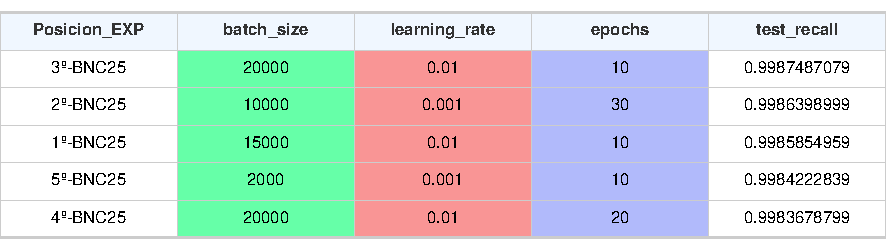
\includegraphics[width=0.9\textwidth]{./img/evaluacion/EVALMCB25.pdf}
    \caption{Resultados de la evaluación del modelo con \textit{n/2} neuronas en la capa oculta siendo \textit{n} el número de atributos de entrada.}
    \label{fig:EVALMCB25}
\end{figure}

Los valores de la métrica \textit{Recall} obtenidos en las evaluaciones del modelo MCB25, son muy altos para todas las configuraciones y la diferencia entre sus valores es del orden de $1e-4$. Estas diferencias pueden deberse a circunstancias no controlables como el estado en el que se encontraba la máquina cuando se realizó la evaluación de los modelos o los pesos aleatorios iniciales que se eligieron en esa ejecución de los \textit{test}.

\subsubsection{MCB49: Modelo de clasifcación binaria con un tamaño de capa oculta igual al número de atributos de entrada que recibe el modelo}
En la Figura \ref{fig:EVALMCB49} se presentan los resultados obtenidos durante las evaluaciones de las cinco configuraciones de hiperparámetros con mejor desempeño, seleccionadas en la fase de búsqueda para la arquitectura del modelo de clasificación binaria que cuenta con una capa oculta de 49 neuronas.

\begin{figure}[H]
    \centering
    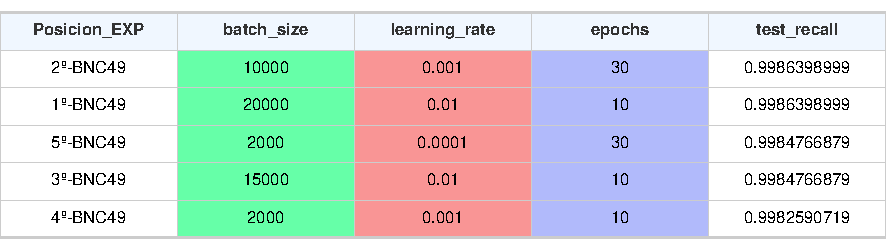
\includegraphics[width=0.9\textwidth]{./img/evaluacion/EVALMCB49.pdf}
    \caption{Resultados de la evaluación del modelo con \textit{n} neuronas en la capa oculta siendo \textit{n} el número de atributos de entrada.}
    \label{fig:EVALMCB49}
\end{figure}

Los valores de la métrica \textit{Recall} obtenidos durante las evaluaciones del modelo MCB49 son consistentemente altos para todas las configuraciones, y las diferencias entre ellos se encuentran en el orden de magnitud de $1e-4$. Estas variaciones podrían atribuirse a factores no controlables, como el estado del sistema al momento de la evaluación o la aleatoriedad en la inicialización de los pesos durante la ejecución de las pruebas.

\subsubsection{MCB98: Modelo de clasifcación binaria con un tamaño de capa oculta igual al doble del número de atributos de entrada que recibe el modelo}
La Figura \ref{fig:EVALMCB98} muestra los resultados obtenidos en las evaluaciones correspondientes a las cinco configuraciones de hiperparámetros que presentaron el mejor desempeño durante la fase de búsqueda, aplicadas a la arquitectura del modelo de clasificación binaria con una capa oculta de 98 neuronas.

\begin{figure}[H]
    \centering
    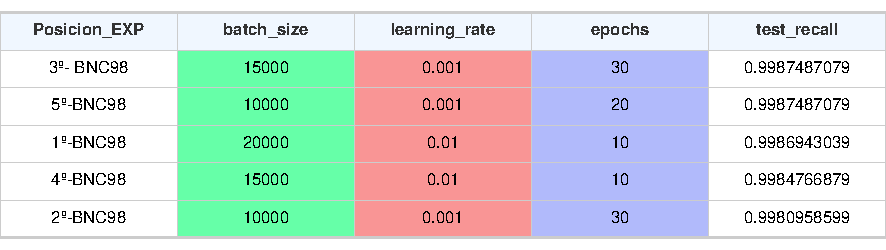
\includegraphics[width=0.9\textwidth]{./img/evaluacion/EVALMCB98.pdf}
    \caption{Resultados de la evaluación del modelo con \textit{2n} neuronas en la capa oculta siendo \textit{n} el número de atributos de entrada.}
    \label{fig:EVALMCB98}
\end{figure}

En las evaluaciones del modelo MCB98, los valores obtenidos para la métrica Recall fueron elevados en todas las configuraciones, con diferencias del orden de $1e-4$. Estas pequeñas variaciones pueden explicarse por factores no controlables, como el estado del sistema en el momento de la evaluación o la inicialización aleatoria de los pesos durante la ejecución de las pruebas.

\subsection{Resultados del modelo de clasificación multiclase}
\section{Análisis de los resultados obtenidos}
\subsection{Modelo de clasificación binaria}

\begin{figure}[H]
    \centering
    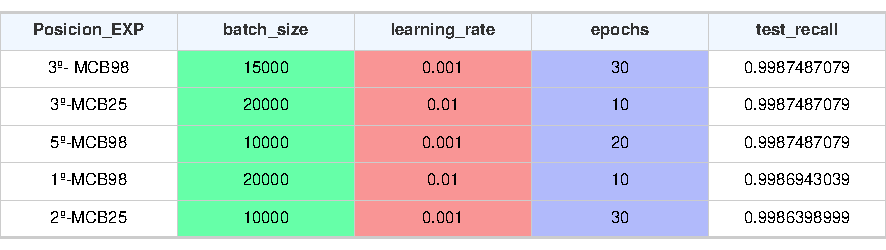
\includegraphics[width=0.9\textwidth]{./img/evaluacion/top5EVALMCB.pdf}
    \caption{Cinco mejores modelos en la fase de evaluación del modelo de clasificación binaria.}
    \label{fig:top5EVALMCB}
\end{figure}

\subsubsection{Fortalezas del modelo de clasificación binaria}
\subsubsection{Debilidades del modelo de clasificación binaria}
\subsection{Modelo de clasificación multiclase}
\subsubsection{Fortalezas del modelo de clasificación multiclase}
\subsubsection{Debilidades del modelo de clasificación multiclase}
